\documentclass[11pt,a4paper]{article}

\usepackage[utf8]{inputenc}
\usepackage[margin=1in]{geometry}
\usepackage{mathptmx} % Times New Roman font for text and math
\usepackage{helvet}
\usepackage{courier}
\usepackage{microtype}
\usepackage{amsmath,amssymb}
\usepackage{graphicx}
\usepackage{listings}
\usepackage{xcolor}
\usepackage{hyperref}
\usepackage{booktabs}
\usepackage{tabularx}
\usepackage{float}
\usepackage{enumitem}
\usepackage{needspace}
\usepackage{setspace}
\usepackage{titlesec}
\usepackage{fancyhdr}
\setstretch{1.2}
\titleformat{\section}{\Large\bfseries}{\thesection}{1em}{}
\titleformat{\subsection}{\large\bfseries}{\thesubsection}{1em}{}
\pagestyle{fancy}\fancyhf{}\fancyhead[L]{Smart Campus Safety \& Risk Grid}\fancyhead[R]{System Documentation}\fancyfoot[C]{\thepage}

% Configure graphicspath so images resolve on Overleaf (root upload) and locally
\graphicspath{{../readme_resources/}{readme_resources/}{images/}{./}}

\hypersetup{
    colorlinks=true,
    linkcolor=blue!80!black,
    citecolor=blue!80!black,
    urlcolor=blue!80!black
}

\definecolor{codegray}{rgb}{0.5,0.5,0.5}
\definecolor{codegreen}{rgb}{0,0.6,0}
\definecolor{backcolour}{rgb}{0.96,0.96,0.96}

\lstset{
    backgroundcolor=\color{backcolour},
    commentstyle=\color{codegreen},
    keywordstyle=\color{blue},
    numberstyle=\tiny\color{codegray},
    stringstyle=\color{red!70!black},
    basicstyle=\ttfamily\footnotesize,
    breakatwhitespace=false,
    breaklines=true,
    captionpos=b,
    keepspaces=true,
    numbers=left,
    numbersep=5pt,
    showspaces=false,
    showstringspaces=false,
    showtabs=false,
    tabsize=2,
    samepage=true
}

\title{}\author{}\date{}

\begin{document}

\begin{titlepage}
\centering
\vspace*{2cm}
{\Huge\bfseries Smart Campus Safety \& Risk Grid (SCS-RG)\par}
\vspace{0.5cm}
{\Large System Documentation\par}
\vspace{0.3cm}
{\large Hardware Design • Software Architecture • API Reference • Risk Fusion Engine\par}
\vfill
{\Large\textbf{Team Clover}\par}
Sadman Islam\\Shah Samin Yasar\\Ahmed Thousif Thisham

\vspace{0.8cm}
Metropolitan University

\vfill

\begin{center}
\renewcommand{\arraystretch}{1.6}
\begin{tabular}{rl}
\textbf{GitHub Repository:} &
\href{https://github.com/amisadman/RoboFusion_Techathon_TeamClover}{github.com/amisadman/RoboFusion\_Techathon\_TeamClover} \\

\textbf{Frontend Dashboard:} &
\href{https://clover-scs-rg.vercel.app/}{clover-scs-rg.vercel.app} \\

\textbf{Backend API:} &
\href{https://robofusion-techathon-teamclover.onrender.com}{robofusion-techathon-teamclover.onrender.com} \\

\textbf{IoT Lab Wokwi:} &
\href{https://wokwi.com/projects/470514529070990337}{wokwi.com/projects/470514529070990337} \\

\textbf{Server Room Wokwi:} &
\href{https://wokwi.com/projects/470509081717871617}{wokwi.com/projects/470509081717871617} \\

\textbf{Data Science Lab Wokwi:} &
\href{https://wokwi.com/projects/470523315735022593}{wokwi.com/projects/470523315735022593}
\end{tabular}
\end{center}

\vfill
\today
\end{titlepage}


% --- PAGE 1: TITLE, CLICKABLE AUTHORS, LINKS, ABSTRACT ---

\thispagestyle{empty}

\newpage

% --- PAGE 2: TABLE OF CONTENTS ---
\thispagestyle{plain}
\tableofcontents
\newpage\section*{Abstract}\large
This document serves as the complete \textbf{System Documentation} for the \textbf{Smart Campus Safety \& Risk Grid (SCS-RG)}. Built for multi-hazard IoT emergency monitoring and campus safety management, SCS-RG integrates ESP32 hardware sensor nodes, a bounded multi-hazard risk fusion engine, real-time WebSocket state streaming, atomic incident priority dispatching, a predictive logistic regression model, and a natural-language incident parsing engine. This document details per-zone hardware circuit diagrams, software architecture specifications, database ER diagrams, mathematically justified risk fusion formulas, and complete REST API endpoint specifications with example payloads.
\normalsize

% --- PAGE 3+: MAIN DOCUMENTATION CONTENT STARTS ---
\section{System Overview \& Software Architecture}

The SCS-RG system is engineered as a decoupled, multi-tiered campus safety grid comprising hardware sensor nodes, an Express/PostgreSQL backend processing engine, and a Next.js 16 command center web interface.

\subsection{Architectural Layering}
\begin{itemize}[leftmargin=*]
    \item \textbf{Hardware Ingestion Layer}: Distributed ESP32 microcontroller nodes sampling Flame, Gas (MQ2), Water Level, and PIR Occupancy telemetry at 10\,Hz.
    \item \textbf{Transport \& Security Layer}: Express.js API gateway enforcing \texttt{X-Zone-Key} microcontroller authentication and session-based Role-Based Access Control (RBAC).
    \item \textbf{Processing Engine Layer}: Bounded Multi-Hazard Risk Fusion Engine, $N=3$ Flame Debounce Filter, Exponential Decay Smoother, Atomic Priority Queue Ranker, Logistic Regression Predictor, and Natural Language Parser.
    \item \textbf{Data Persistence Layer}: PostgreSQL relational database managed via Prisma ORM for ACID transactional integrity.
    \item \textbf{Realtime Distribution Layer}: Socket.io WebSocket server broadcasting real-time state changes (\texttt{zone:state}, \texttt{priority:update}, \texttt{incident:opened}) to active operator dashboards.
    \item \textbf{Presentation Layer}: Next.js 16 App Router interface featuring responsive dual-theme command console, live zone grid, dispatch ledger, and Recharts analytics.
\end{itemize}

\subsection{Software Architecture Diagram}
\begin{figure}[H]
\centering
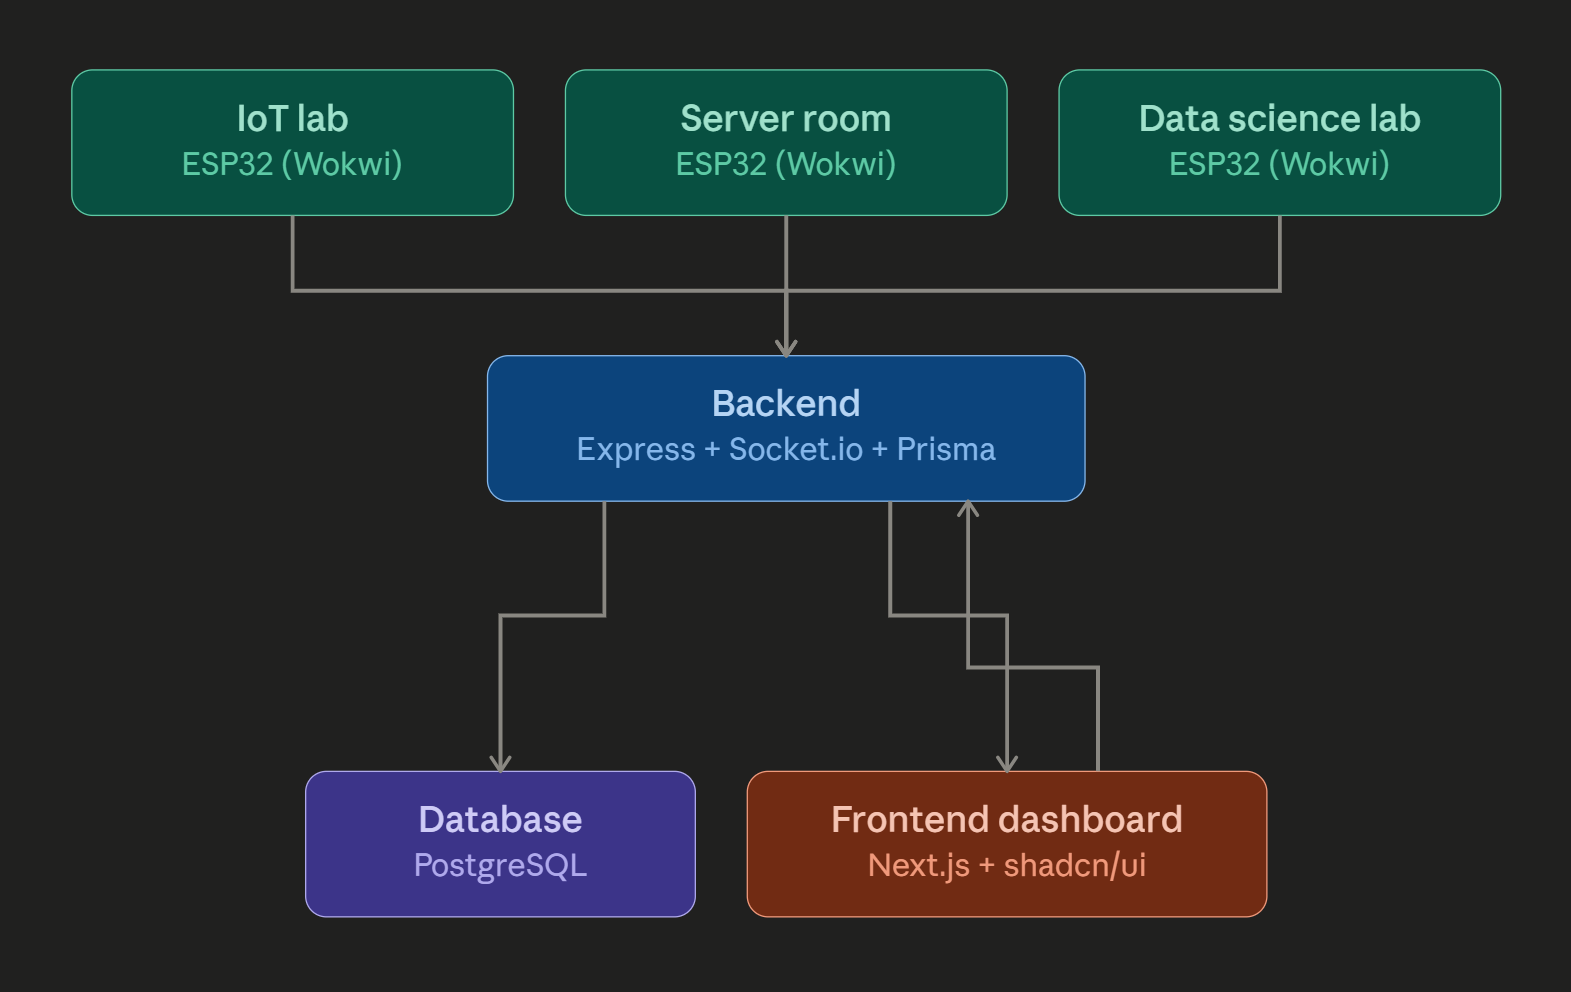
\includegraphics[width=0.95\textwidth]{system_architecture.png}
\caption{System Component Architecture \& High-Level Layering}
\end{figure}

---

\section{Hardware Sensor Circuit Diagrams (Per Zone)}

SCS-RG deploys three dedicated hardware sensor nodes monitoring distinct campus zones:

\subsection{1. IoT Lab Node Circuit Diagram}
Monitors soldering stations, chemical storage, and prototype hardware development. Wired with ESP32, IR Flame Sensor (Pin 34), MQ2 Gas Sensor (Pin 35), Water Level Sensor (Pin 32), PIR Motion Sensor (Pin 33), Status LED (Pin 2), Buzzer (Pin 25), and Emergency Relay Cutoff (Pin 26).\\
\small \textbf{Live Wokwi Simulation:} \href{https://wokwi.com/projects/470514529070990337}{https://wokwi.com/projects/470514529070990337}

\begin{figure}[H]
\centering
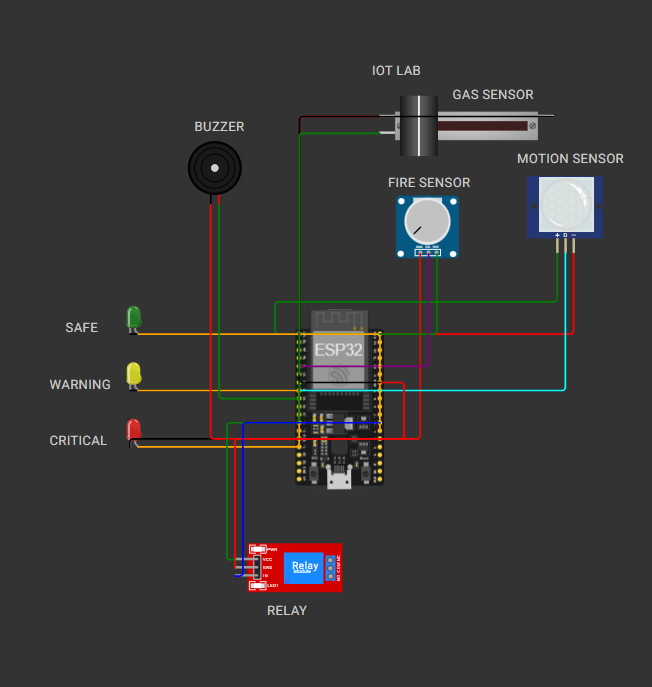
\includegraphics[width=0.70\textwidth]{iot_lab.png}
\caption{IoT Lab Node Hardware Circuit Diagram}
\end{figure}

\subsection{2. Server Room Node Circuit Diagram}
Monitors high-density server racks, power distribution units, and electrical switches. Optimized for electrical fire detection and cooling fluid leak monitoring.\\
\small \textbf{Live Wokwi Simulation:} \href{https://wokwi.com/projects/470509081717871617}{https://wokwi.com/projects/470509081717871617}
\begin{figure}[H]
\centering
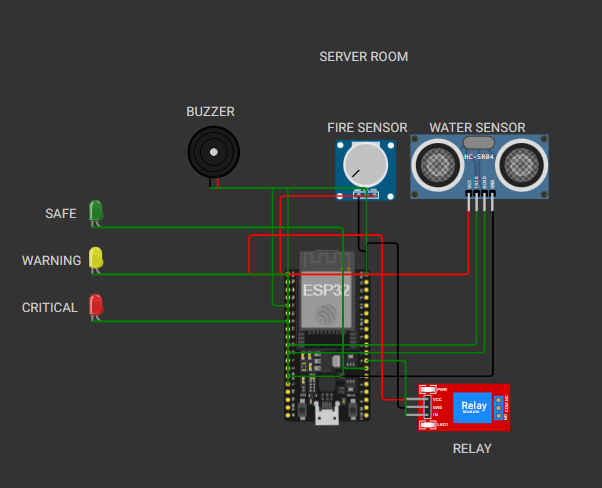
\includegraphics[width=0.70\textwidth]{server_room.png}
\caption{Server Room Node Hardware Circuit Diagram}
\end{figure}

\subsection{3. Data Science Lab Node Circuit Diagram}
Monitors high-performance computing clusters and student workstation clusters.\\
\small \textbf{Live Wokwi Simulation:} \href{https://wokwi.com/projects/470523315735022593}{https://wokwi.com/projects/470523315735022593}

\begin{figure}[H]
\centering
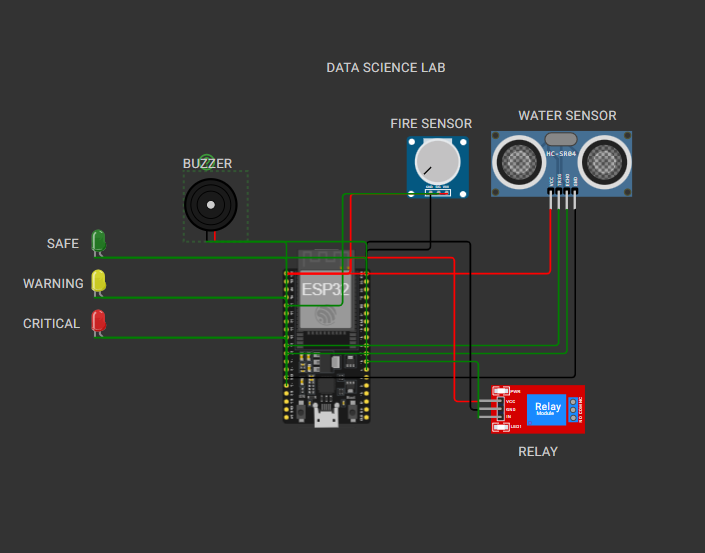
\includegraphics[width=0.70\textwidth]{data_science_lab.png}
\caption{Data Science Lab Node Hardware Circuit Diagram}
\end{figure}

---

\section{Mathematical Risk Calculation Formula \& Weight Justifications}

The core safety engine evaluates overall zone risk using a \textbf{Bounded Multi-Hazard Risk Fusion Engine}. It computes a single scalar Risk Score $R \in [0.0, 100.0]$.

\subsection{Mathematical Fusion Formula}
\begin{equation}
R = \min\left(100.0, \, w_{\text{fire}} \cdot x_{\text{fire}} + w_{\text{gas}} \cdot x_{\text{gas}} + w_{\text{water}} \cdot x_{\text{water}} + w_{\text{occ}} \cdot x_{\text{occ}}\right)
\end{equation}

Where $x_i \in [0.0, 1.0]$ represents the normalized sensor input after dynamic ADC resolution scaling:
\begin{equation}
x_{\text{sensor}} = \min\left(1.0, \frac{\text{raw\_adc}}{\text{MaxADC}(\text{raw\_adc})}\right), \quad \text{MaxADC} = \begin{cases} 4095.0 & \text{if 12-bit ESP32} \\ 1023.0 & \text{if 10-bit Arduino} \end{cases}
\end{equation}

\subsection{Hazard Weight Justifications}
\begin{table}[H]
\centering
\begin{tabularx}{\textwidth}{l c X}
\toprule
\textbf{Hazard Component} & \textbf{Weight ($w_i$)} & \textbf{Engineering \& Safety Justification} \\
\midrule
Fire ($w_{\text{fire}}$) & 65.0 & \textbf{Critical Life Safety Threat}: Thermal combustion spreads rapidly and presents immediate catastrophic risk to life and physical assets. Demands top weighting. \\
Gas ($w_{\text{gas}}$) & 65.0 & \textbf{Explosion Risk}: Combustible gas accumulation (MQ2) creates severe explosion hazards in confined lab spaces. Equal priority to fire. \\
Water ($w_{\text{water}}$) & 30.0 & \textbf{Electrical Short \& Equipment Submersion}: Fluid leaks cause electrical shorts and equipment failure. \\
Occupancy ($w_{\text{occ}}$) & 25.0 & \textbf{Human Life Multiplier}: Presence of occupants elevates emergency dispatch priority to ensure rapid evacuation. \\
\bottomrule
\end{tabularx}
\caption{Hazard Weights and Engineering Justifications}
\end{table}

\subsection{Flame Debounce Filter ($N=3$ Cycles) \& Decay Smoothing}
To eliminate optical noise, raw flame signals must pass a 3-cycle window before triggering full activation. When hazards subside, active risk score decays gradually by $5.0\text{ points/cycle}$:
\begin{equation}
R_{\text{active}}(t) = \max\left(R_{\text{fusion}}(t), \, R_{\text{active}}(t-1) - 5.0\right)
\end{equation}

\subsection{Zone State Classification Thresholds}
\begin{equation}
\text{State} = \begin{cases}
\text{OFFLINE} & \text{if sensor health is disconnected OR silent } > 10\text{s} \\
\text{CRITICAL} & \text{if } R_{\text{active}} \ge 65.0 \\
\text{WARNING} & \text{if } 30.0 \le R_{\text{active}} < 65.0 \\
\text{SAFE} & \text{if } R_{\text{active}} < 30.0
\end{cases}
\end{equation}

---

\section{Database Schema \& Entity-Relationship Diagram}

The persistence layer uses PostgreSQL managed via Prisma ORM.

\subsection{Database Entity-Relationship (ER) Diagram}
The complete database ER diagram detailing entity relationships across \texttt{Zone}, \texttt{Reading}, \texttt{Incident}, \texttt{IncidentTransition}, and \texttt{User}:

\begin{figure}[H]
\centering
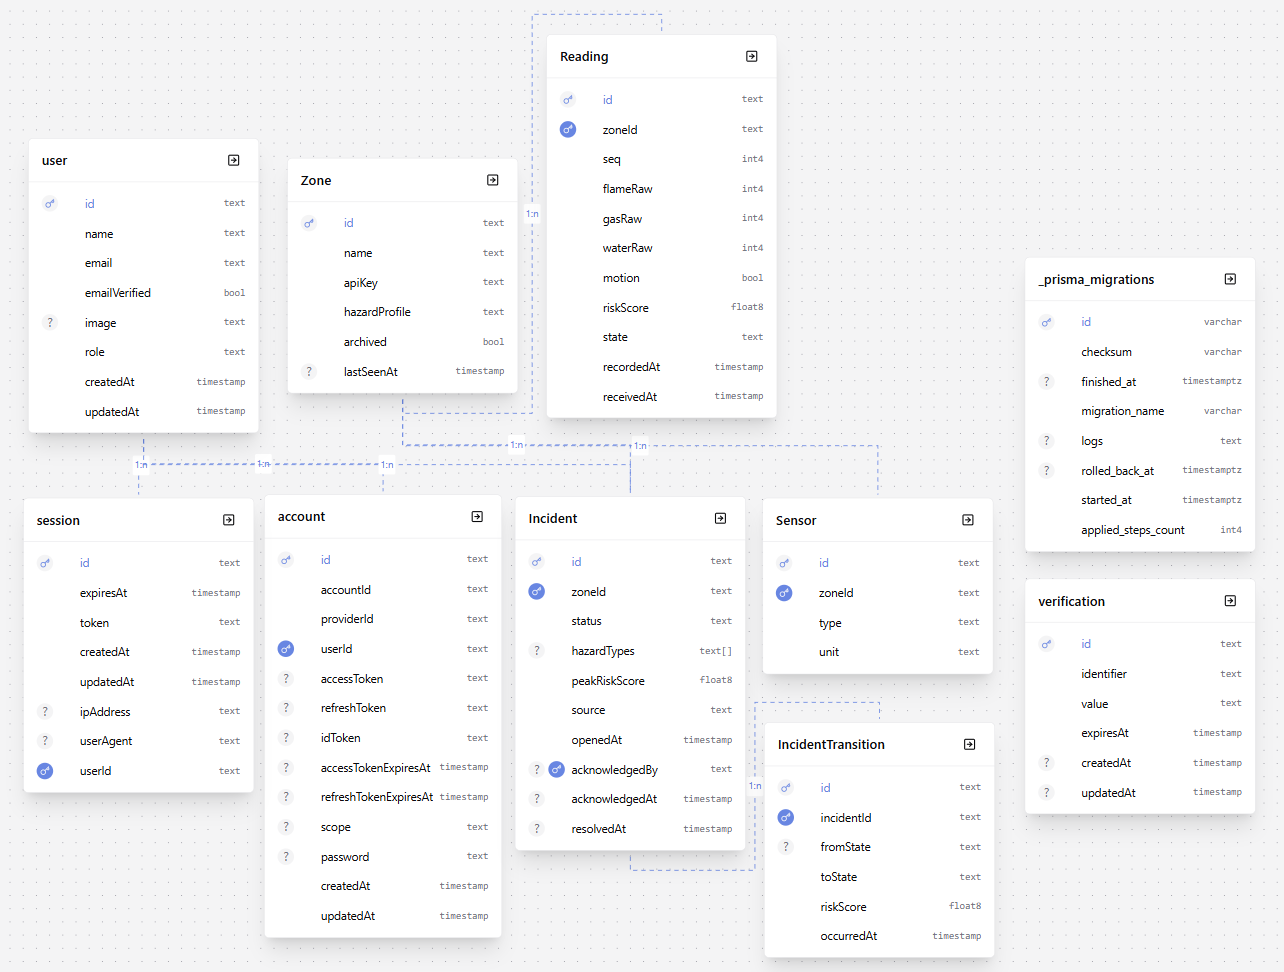
\includegraphics[width=1\textwidth]{db_schema.png}
\caption{Database Entity-Relationship (ER) Diagram}
\end{figure}

---

\newpage
\section{API Endpoints Reference with Example Requests \& Responses}

All API responses follow a unified JSON envelope format. Below are the complete, unbroken payload examples for each endpoint.

\subsection{1. Microcontroller Telemetry Ingestion (\texttt{POST /api/readings})}
\paragraph{Request Header}: \texttt{X-Zone-Key: key\_server\_room\_456}

\needspace{14\baselineskip}
\begin{lstlisting}[language=json, samepage=true]
POST /api/readings HTTP/1.1
Host: robofusion-techathon-teamclover.onrender.com
Content-Type: application/json
X-Zone-Key: key_server_room_456

{
  "zone_id": "server_room",
  "seq": 142,
  "timestamp_ms": 1721985430000,
  "sensors": {
    "flame_raw": 3200,
    "gas_raw": 1800,
    "water_raw": 150,
    "motion": true
  },
  "sensor_health": { "flame": "ok", "gas": "ok", "water": "ok", "motion": "ok" }
}
\end{lstlisting}

\needspace{14\baselineskip}
\paragraph{Response (200 OK)}:
\begin{lstlisting}[language=json, samepage=true]
{
  "success": true,
  "message": "Reading ingested successfully",
  "data": {
    "accepted": true,
    "state": "CRITICAL",
    "risk_score": 73.2,
    "commands": { "led": "red", "buzzer": true, "relay_cutoff": true },
    "server_seq_ack": 142
  }
}
\end{lstlisting}

\needspace{14\baselineskip}
\subsection{2. Get All Active Zones (\texttt{GET /api/zones})}
\paragraph{Response (200 OK)}:
\begin{lstlisting}[language=json, samepage=true]
{
  "success": true,
  "message": "Zones retrieved successfully",
  "data": [
    {
      "zone_id": "server_room",
      "name": "Server Room 101",
      "hazard_profile": "High density electrical & server racks",
      "state": "CRITICAL",
      "risk_score": 73.2,
      "occupied": true,
      "last_seen_at": "2026-07-26T14:30:00.000Z"
    }
  ]
}
\end{lstlisting}

\needspace{14\baselineskip}
\subsection{3. Priority Dispatch Queue (\texttt{GET /api/priority})}
\paragraph{Response (200 OK)}:
\begin{lstlisting}[language=json, samepage=true]
{
  "success": true,
  "message": "Priority queue retrieved successfully",
  "data": {
    "ranked": [
      {
        "zone_id": "server_room",
        "rank": 1,
        "risk_score": 73.2,
        "occupied": true,
        "seconds_critical": 45,
        "reason": "risk 73.2, occupied, critical 45s",
        "source": "sensor",
        "incident_id": "clx82910a0001"
      }
    ]
  }
}
\end{lstlisting}

\needspace{14\baselineskip}
\subsection{4. Atomic Incident Acknowledgment (\texttt{POST /api/incidents/:id/ack})}
\paragraph{Response (200 OK)}:
\begin{lstlisting}[language=json, samepage=true]
{
  "success": true,
  "message": "Incident acknowledged successfully",
  "data": {
    "success": true,
    "statusCode": 200,
    "incident_id": "clx82910a0001",
    "acknowledged_by": "usr_admin_123",
    "acknowledged_at": "2026-07-26T14:31:00.000Z"
  }
}
\end{lstlisting}

\needspace{16\baselineskip}
\subsection{5. Natural Language Incident Reporting (\texttt{POST /api/bonus/nl-report})}
\paragraph{Request Payload}:
\begin{lstlisting}[language=json, samepage=true]
POST /api/bonus/nl-report HTTP/1.1
Content-Type: application/json

{
  "text": "Heavy smoke and electrical fire smell coming from the server room rack 4"
}
\end{lstlisting}

\paragraph{Response (200 OK)}:
\begin{lstlisting}[language=json, samepage=true]
{
  "success": true,
  "message": "Natural language report processed successfully",
  "data": {
    "parsed": true,
    "input_text": "Heavy smoke and electrical fire smell coming from the server room rack 4",
    "extracted_signal": {
      "zone_id": "server_room",
      "hazard_type": "fire",
      "estimated_severity": "CRITICAL"
    },
    "validation_gate": "passed",
    "incident_id": "clx99201b0002"
  }
}
\end{lstlisting}

\end{document}
